The hypothesis of this research is that "\textit{Individual and population level air pollutant exposure can be estimated using time-activity surveys, GIS and routing tools, coupled with high resolution spatio-temporal air quality models, facilitating a greater understanding of the health impacts of air pollution and how public health risks can be reduced}". The research objectives that will need to be met to achieve this goal are as follows:

\begin{enumerate}
\item Reconstruct the time-space activity of London's population
\item Link modelled air quality, estimate exposure, and compare with traditional methods
\item Refine the models estimates of London Underground exposure
\item Evaluate the results
\end{enumerate}

In more detail I will model the movements of the subject's in the TfL dataset, reconstruct their days on a fine temporal and spatial scale, and then use this data in conjunction with a novel exposure model. The air quality input will be a CMAQ-UK model (see Section \ref{sec:cmaq_urban}). The results of the model will allow interrogation of exposure by individual, or grouped by various demographics, which will enable epidemiologists to increase their understanding of exposure miss-classification. Results will be compared to static modelling approaches of the type discussed in Section \ref{sec:staticexposurehealth}. The model will then be improved with personal monitoring on the London Underground, before an introduction to validation/testing of the results will be undertaken. The objectives will be met by following the work-plan below.

\section{Modelling Londoners movements}

\textbf{Aim:} Create a model of Londoners daily movements based upon the London Transport Demand Survey \\
\textbf{Objectives:}

\begin{enumerate}
\item Explore the LTDS dataset and identify key data
\item Move data from local Microsoft Access database into a PostgreSQL + PostGIS database
\item Clean data
\item Complete modal specific routing (interrogation, querying, storage) between origin and destinations
\item Quality check the routing results and do further data cleaning
\item Create and populate final dynamic location database table
\item Analysis of results
\end{enumerate}

\section{Dynamic exposure modelling}

\textbf{Aim:} Model exposure to PM$_{2.5}$ and NO$_{2}$ of the LTDS-X subjects, and compare  with traditional exposure models \\
\textbf{Objectives:}

\begin{enumerate}
\item Link data to CMAQ-Urban UK, incorporate IO ratios and micro-environmental factors (The 'LHEM')
\item Create a postcode comparison dataset
\item Create a address-point comparison dataset
\item Create a monitoring sites comparison dataset
\item Analysis and comparison of results
\end{enumerate}

Thus far, these aims cover the first half of the conceptual exposure model shown in Figure \ref{fig:james_exposure_diagram} (which is repeated here for convenience). 

\begin{figure}[H]
\centering
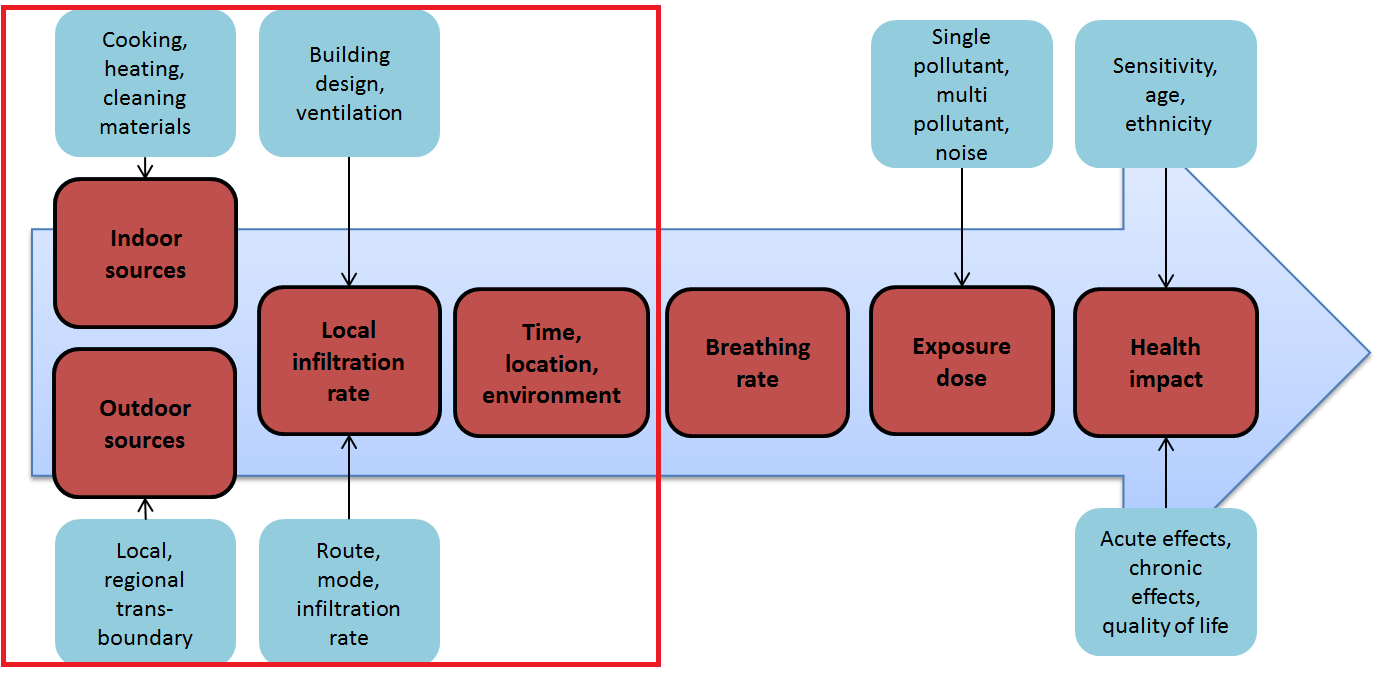
\includegraphics[scale=0.4]{james_exposure_diagram_v2}
\caption{A conceptual dynamic exposure model}
\label{fig:james_exposure_diagram_v2}
\end{figure}

The following two sections will be on improving exposure estimates, and evaluating them respectively.

\section{Exposure to \texorpdfstring{PM$_{2.5}$}{} on the London Underground}

\textbf{Aim:} Create an exposure model for PM$_{2.5}$ on the London Underground \\
\textbf{Objectives:}

\begin{enumerate}
\item Measure PM$_{2.5}$ across the London Underground network
\item Transcribe a time-location diary and link to pollutant data
\item Import other relevant data
\item Analyse data to characterise PM$_{2.5}$ on the London Underground
\end{enumerate}

\section{Evaluating dynamic exposure models}

\textbf{Aim:} Develop an understanding of methods to evaluate predictions of exposure from hybrid models \\
\textbf{Objectives:}

\begin{enumerate}
    \item Establish how to use mobile monitoring equipment to replicate static monitoring site datasets (which are used for air quality model evaluation)
    \item Collect mobile monitoring data representative of a journey from the LHEM
    \item Model exposure of this journey using LHEM methodology
    \item Compare the monitored and modelled exposures
\end{enumerate}